\section{Segmentation (V8, V9)}
  Segmentation subdivides an image into its constituent (zusammengehörend) regions or object. 
  $\Rightarrow$ One of the most
  difficult tasks in ImPro. Usually, post processing is required to identify and potentially label
  objects.
  
  Problems: Uneven illumination, noise
  
  \skriptsubsection{Edge Based Segmentation}{692}
    Aim: Finding borders or lines of objects: Contours, similarity of adjacent pixels can be detected.
    
    3 Steps:
    \begin{aufzaehlung}
      \item Preprocessing \& smoothing: noise reduction, small object removal, intensity transformations
      \item Edge point detection: Edge pixel detection, derivatives in X,Y direction with 1st and/or 2nd order filters (Laplacian)
      \item Postprocessing (localize edges): thresholding, thinning, zero crossings of 2nd order derivative
    \end{aufzaehlung}
    
    \skriptsubsubsection{Line Detection}{697}
      See spatial filters (Section \ref{sec:filter_types}) for Laplacian Sobel, Prewitt, \ldots
       
    \skriptsubsubsection{Point detection}{696}
      Point detection: Use 2nd order derivation (Laplacian): 
      $\nabla^2 f(x,y) = \frac{\delta^2 f}{\delta x^2} + \frac{\delta^2f}{\delta y^2} = 
      \left(f(x+1,y)+f(x-1,y)-2f(x,y)\right) + \left(f(x,y+1)+f(x,y-1)-2f(x,y)\right)$
      $H_{3 \times 3} = \begin{bmatrix}
        1 & 1 & 1 \\
        1 & -8 & 1 \\
        1 & 1 & 1 \\
      \end{bmatrix}$
    
    \skriptsubsubsection{Marr-Hildreth Edge Detector}{714}
      Intensity changes are not
      independent of image scale and so their detection requires the use of operators of different
      sizes; and that a sudden intensity change will give rise to a peak or trough (Mulde) in the first 
      derivative or equivalently a zero crossing in the second derivative.
      
      The operator for smoothing and Laplacian is called \em Laplacian of a Gaussian (LoG) \em or \em Mexican hat\em:
      $\nabla^2G(x,y) = \left( \frac{x^2 + y^2 2\sigma^2}{\sigma^4} e^{-\frac{x^2+y^2}{2\sigma^2}} \right)$
      with $\sigma$ being the standard deviation of the image.
      
      The size of the filter ($n \times n$) should be an odd integer with $n > \ceil(6 \sigma)$.
     
      Discussion:
      \begin{liste}
      	\item Strong smoothing (sharp edges might be lost)
      	\item Mostly closed edges
      	\item Sensitive to noise
      	\item Post-processing (zero-cross detection) required
      \end{liste}
  
    \skriptsubsubsection{Canny Edge Detector}{714}
      Use first order derivative in both directions.
      
      \begin{aufzaehlung}
      	\item Smooth image with Gaussian
      	\item Compute gradient (Sobel, Prewitt, \ldots) in both directions
      	\item Non-maxima suppression to gradient magnitude image (alles was nicht max ist, unterdrücken)
      	\item Double thresholding:
      	  \begin{liste}
      	  	\item Pixels with $f(x,y) > T_1$ belong to edge (strong edge pixels)
      	  	\item Pixels with $T_1 > f(x,y) > T_2$ belong to edge when there is a strong edge pixel
      	  	in the $8\times 8$ neighbourhood (weak edge pixels)
      	  \end{liste}
      	\item If necessary, edge thinning
      \end{aufzaehlung}
      This algo is considerably slower but performs better than Marr-Hildreth.
      
    \skriptsubsubsection{Edge Linking and Boundary Detection}{725}
      Edges are going to be linked together as they are typically not connected.
      
      \subsubsubsection{Local Processing}
        \begin{aufzaehlung}
        	\item Compute gradient $\nabla f= \begin{bmatrix}g_x\\g_y\end{bmatrix}$ (Sobel, Prewitt,\ldots)
          \item Compute magnitude $M(x,y) = \sqrt{g_x^2+g_y^2} \approx |g_x| + |g_y|$ and angle $\varphi(x,y) = \arctan(g_y/g_x)$
        	\item Set neighbour pixel (8-connected neighbours) at $(s,t)$ of pixel $(x,y)$ as edge
        	pixel when $|M(s,t) - M(x,y)| \leq m_0$ and $|\varphi(s,t) - \varphi(x,y)| \leq \varphi_0$
        	\item If necessary: Thinning and remove single edge pixels
        \end{aufzaehlung}
        
      \subsubsubsection{Global Processing}
        Find lines instead of simple edges
        
      \subsubsubsection{Hough Transform}
        See later\ldots
        
      \subsubsubsection{Edge Linking}
    
  \skriptsubsection{Thresholding}{738}
    \skriptsubsubsection{Definitions}{738}
      \begin{liste}
      	\item Global threshold: One threshold depending on intensity $T = T(f(x,y))$
      	\item Local threshold: Threshold may also depend on neighbourhood (e.g. grey level average, variance, \ldots)
      	  $T = T(f(x,y), p(x,y))$
      	\item Dynamic or variable or adaptive threshold: Depending on position: $T = T(x,y, f(x,y))$
      	\item Hysteresis thresholding: 1. Global threshold with $T_H$, 2. Threshold in the 
      	$k$-connected (e.g. $k=4,8$) neighborhood of all pixels detected in (1) with lower threshold $T_L$.
      \end{liste}
      
      Problems of thresholding: Noise, illumination
      
    \skriptsubsubsection{Basic Method}{741}
      \begin{aufzaehlung}
      	\item Initial $T$ (e.g. middle point between 2 maxima)
      	\item Segment image with $T$ into $G_1 \leq T$, $G_2 > T$
      	\item Compute average intensity value $m_1$, $m_2$ in $G_1$, $G_2$
      	\item Compute new threshold value: $T = \frac12 (m_1 + m_2)$
      	\item Repeat steps 2..4 until the difference of the $T$s is smaller than a constant $\epsilon$
      \end{aufzaehlung}
  
    \skriptsubsubsection{Otsu's Method}{742}
      Statistical approach to find best threshold.
      \begin{aufzaehlung}
      	\item Compute the normalized histogram of the input image. Denote the components of the 
      	  histogram by $p_i$, $i=0,1,\ldots,L-1$.
      	\item Compute cumulative sums: $P(k) = \sum_{i=0}^k p(i)$ for $k=0,1,\ldots,L-1$
      	\item Compute cumulative means: $m(k) = \sum_{i=0}^k i p(i)$ for $k=0,1,\ldots,L-1$
      	\item Compute global intensity mean: $m_G = \sum_{i=0}^{L-1} i p(i)$
      	\item Compute between-class variance: $\sigma_B^2(k) = \frac{(m_G P_1(k) - m(k))^2}{P_1(k)(1-P_1(k))}$ 
      	  for $k=0,1,\ldots,L-1$
      	\item Obtain Otsu threshold $k^* = \max_{k = 0,1,\ldots,L-1} \sigma_B^2(k)$. If max is not unique,
      	  average these $k$s.
      \end{aufzaehlung}
      Otsu is not always better than basic approach!
      
    \skriptsubsubsection{Smoothing}{747}
      Again, smoothing might improve results when noise is a problem.
      
    \skriptsubsubsection{Edges}{749}
      Improving the shape of histograms by considering only thoe pixels that lie on or near the edges
      between the objects and the background. $\Rightarrow$ less dependency of size of objects and background.
      \begin{aufzaehlung}
      	\item Find edges
      	\item Threshold edge image $\rightarrow$ binary image
      	\item Mask original image with thresholded edge image
      	\item Compute the histogram using only the pixels in the origianl image that correspond to 
      	  the locations of the 1-valued pixels in image from step 3. Evaluate threshold with the 
      	  basic method, Otsu, etc.
        \item Segment original image using this threshold
      \end{aufzaehlung}
      
    \skriptsubsubsection{Adaptive Thresholding}{756}
      \begin{tabular}{ll}
        \parbox{13cm}{
          Subdivide image and compute threshold for every region. Hint: 
          Regions must consist of both object and background, otherwise the thresholding would not 
          work and only distinguish between noise. Therefore, regions must be not too big and not too small.
      
    \skriptsubsubsection{Multivariable Thresholds}{761} 
      Use RGB color information for thresholding: $\bm z = [r, g, b]^T$. This is a 3D vector which 
      can also be referred as \em voxel \em (volume element).
      }
        & \parbox{6cm}{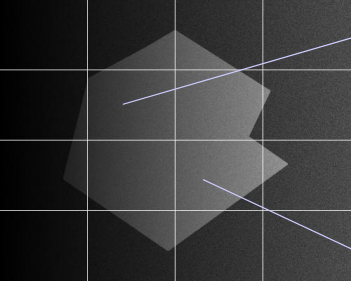
\includegraphics[width=5cm]{./images/adaptive_thresholding.png}}
      \end{tabular}

  \skriptsubsection{Region Based Segmentation}{763}
    Find boundaries between regions directly (in contrast to thresholding) according to some
    criteria (gray level, color, texture, form, \ldots). This is more efficient in terms of noisy
    and blurred images.
  
    \skriptsubsubsection{Region Growing}{763}
      \begin{enumerate}
      	\item Find seed points in input image $f(x,y)$ (e.g. with a very high threshold): $S(x,y)$
      	\item Morphological erosion of $S(x,y)$ to reduce connected components to 1 pixel
      	\item Calculate predicate: E.g. similarity in intensity (intensity threshold) on $f(x,y)$. 
      	  This leads to $f_Q(x,y)$ \todo{check}
      	\item Append found values to seed image and label every connected area.
      \end{enumerate}
      Starting with seed points, grow regions according to some ``criteria'' as mentioned above.
    
    
    \skriptsubsubsection{Splitting and Merging}{766}
      Instead of growing regions from seed points, this strategy grows from arbitrary disjoint regions.
      
      \begin{enumerate}
      	\item Split into four disjoint quadrants any region $R_i$ for which $Q(R_i)=FALSE$ ($Q(R_i)$ 
      	  is the predicate, pixels belonging to object)
      	\item Split all regions again into disjoint regions (if possible)
      	\item End splitting when no more splitting is possible
      \end{enumerate}
    
    \skriptsubsection{Watersheds}{769}
    \begin{minipage}{4cm}
      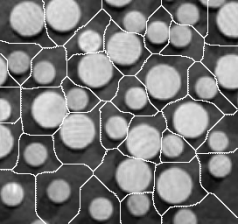
\includegraphics[width=4cm]{./images/morphology_watersheds.png}
    \end{minipage}
    \hspace{0.5cm}
    \begin{minipage}{14.5cm}
      The image can be viewed as a 3D relief with local minima. When ``flooding'' from these minima
      step by step and the ``water'' merges between two regions, a ``dam'' (Damm) can be built. These
      dams (watersheds/Wasserscheiden) are the dividers between regions.
      \begin{liste}
      	\item Use when uniform regions are searched
      	\item Problems: Oversegmentation due to noise or non-uniform regions.
      	\item Possible solutions:
          \begin{liste}
          	\item Smoothing (as always) but with relatively large kernels
          	\item Apply watershed transformation to gradient image (often still oversegmentation $\Rightarrow$ smoothing)
          	\item Use markers as starting point (e.g. shortest distance between black and white pixels)
          \end{liste}
      \end{liste}
    \end{minipage}
      
      